%%%%%%%%%%%%%%%%%%%%%%%%%%%%%%%%%%%%%%%%%%%%%%%%%%%%%%%%%%%%%%%%%%%%%%%%%%%%%%%%
%% ************************************************************************** %%
%% *                                Settings                                * %%
%% ************************************************************************** %%
%%%%%%%%%%%%%%%%%%%%%%%%%%%%%%%%%%%%%%%%%%%%%%%%%%%%%%%%%%%%%%%%%%%%%%%%%%%%%%%%
\documentclass{ece}
\loadglsentries{gls}
\usepackage{tabto}
\usepackage{tabularx}
\usepackage{floatrow}
\newfloatcommand{capbtabbox}{table}[][\FBwidth]
%\usepackage{blindtext}
\glsaddall
\addbibresource{reference}
\usepackage[flushleft]{threeparttable}
\usepackage[autostyle=false, style=english]{csquotes}
\MakeOuterQuote{"}


%%%%%%%%%%%%%%%%%%%%%%%%%%%%%%%%%%%%%%%%%%%%%%%%%%%%%%%%%%%%%%%%%%%%%%%%%%%%%%%%
% Make sure the following block contains the correct information               %
%%%%%%%%%%%%%%%%%%%%%%%%%%%%%%%%%%%%%%%%%%%%%%%%%%%%%%%%%%%%%%%%%%%%%%%%%%%%%%%%
\reporttitle{Netflix Challenge: Movie Rating Prediction}
\employername{CSE-2525 Data Mining}
\employerstreetaddress{Thomas Abeel, Gosia Migut}
\authorname{Yanqing Wu}
\studentnumber{5142571}
\userid{yanqingwutudelft}
\program{Exchanged Computer Engineering}
%%%%%%%%%%%%%%%%%%%%%%%%%%%%%%%%%%%%%%%%%%%%%%%%%%%%%%%%%%%%%%%%%%%%%%%%%%%%%%%%
% end of information block...                                                  %
%%%%%%%%%%%%%%%%%%%%%%%%%%%%%%%%%%%%%%%%%%%%%%%%%%%%%%%%%%%%%%%%%%%%%%%%%%%%%%%%

\begin{document}
%\blindtext
%%%%%%%%%%%%%%%%%%%%%%%%%%%%%%%%%%%%%%%%%%%%%%%%%%%%%%%%%%%%%%%%%%%%%%%%%%%%%%%%
%% ************************************************************************** %%
%% *                               Title Page                               * %%
%% ************************************************************************** %%
%%%%%%%%%%%%%%%%%%%%%%%%%%%%%%%%%%%%%%%%%%%%%%%%%%%%%%%%%%%%%%%%%%%%%%%%%%%%%%%%

\maketitle

%%%%%%%%%%%%%%%%%%%%%%%%%%%%%%%%%%%%%%%%%%%%%%%%%%%%%%%%%%%%%%%%%%%%%%%%%%%%%%%%
%% ************************************************************************** %%
%% *                           Table of Contents                            * %%
%% ************************************************************************** %%
%%%%%%%%%%%%%%%%%%%%%%%%%%%%%%%%%%%%%%%%%%%%%%%%%%%%%%%%%%%%%%%%%%%%%%%%%%%%%%%%

\tableofcontents

%%%%%%%%%%%%%%%%%%%%%%%%%%%%%%%%%%%%%%%%%%%%%%%%%%%%%%%%%%%%%%%%%%%%%%%%%%%%%%%%
%% ************************************************************************** %%
%% *                            List of Figures                             * %%
%% ************************************************************************** %%
%%%%%%%%%%%%%%%%%%%%%%%%%%%%%%%%%%%%%%%%%%%%%%%%%%%%%%%%%%%%%%%%%%%%%%%%%%%%%%%%

\listoffigures

%%%%%%%%%%%%%%%%%%%%%%%%%%%%%%%%%%%%%%%%%%%%%%%%%%%%%%%%%%%%%%%%%%%%%%%%%%%%%%%%
%% ************************************************************************** %%
%% *                             List of Tables                             * %%
%% ************************************************************************** %%
%%%%%%%%%%%%%%%%%%%%%%%%%%%%%%%%%%%%%%%%%%%%%%%%%%%%%%%%%%%%%%%%%%%%%%%%%%%%%%%%

\listoftables

%%%%%%%%%%%%%%%%%%%%%%%%%%%%%%%%%%%%%%%%%%%%%%%%%%%%%%%%%%%%%%%%%%%%%%%%%%%%%%%%
%% ************************************************************************** %%
%% *                                  Body                                  * %%
%% ************************************************************************** %%
%%%%%%%%%%%%%%%%%%%%%%%%%%%%%%%%%%%%%%%%%%%%%%%%%%%%%%%%%%%%%%%%%%%%%%%%%%%%%%%%

\body

\section{Introduction}

The report, entitled ``Netflix Challenge: Movie Rating Prediction'', is prepared as my Challenge report for the course CSE2525-Data Mining at the Technische Universiteit Delft.
The purpose of this report is to develop a recommendation system for predicting movie ratings.
The goal of the recommendation system is to achieve Root Mean Square Error (RMSE) as small as possible on an unseen dataset.

\subsection{Netflix Datasets}

\begin{table}[ht!]
    \caption[The Basic Information of Provided Data Sets]{The Basic Information of Provided Data Sets}
    \label{tab:table-1}
    \centering
    \begin{tabular*}{\textwidth}{@{\extracolsep{\fill}}lllllS[table-format=5.2]}	
    	% l=left-justified column, c=centered column, r=right-justified column
        % 4.4 means 4 digits before and after the decimal point	
        \hline	
        \textbf{Dataset} 
        	& \multicolumn{1}{c}{\textbf{Fields}} & \multicolumn{1}{c}{\textbf{Mean}} 
            & \multicolumn{1}{c}{\textbf{Std.}} & \multicolumn{1}{c}{\textbf{Min \& Max}} \\	
        \hline	
        % ~ gives space	
        users
            & gender
            & 0.72
            & 0.45
        	& \begin{tabular}{@{}l@{}} 0.00 \\ 1.00 \end{tabular}
\\
        	& age
        	& 30.64
        	& 12.90
        	& \begin{tabular}{@{}l@{}} 1.00 \\ 56.00 \end{tabular}
\\
        	& profession
        	& 8.15
        	& 6.33
        	& \begin{tabular}{@{}l@{}} 0.00 \\ 20.00 \end{tabular}
\\      movies
        	& year
        	& 1985.81
        	& 16.91
        	& \begin{tabular}{@{}l@{}} 1919.00 \\ 2000.00 \end{tabular}
\\
			& title (string)
			& -
			& -
			& -
\\		ratings
			& rating
			& 3.58
			& 1.12
			& \begin{tabular}{@{}l@{}} 1.00 \\ 5.00 \end{tabular}
\\      \hline	
   \end{tabular*}
   \begin{tablenotes}
     \item In users - `gender', `0' and `1' indicates female users and male users, respectively;
     \item In movies - `year', only non-zero entries are considered.
   \end{tablenotes}
\end{table}

Three datasets are provided for training, as described in \Cref{tab:table-1}.
There is a total of 910,190 ratings, which were given by 6,040 users and 3,706 movies.
The rest `predictions.csv' file is used for final testing, which contains only `userID` and `movieID' for each entry.
There is a total of 90,019 entries in `predictions.csv' to be predicted and the result is put on Kaggle to determine RMSE score.


\section{Methodology}

Data interpretation was first conducted at the beginning of the Challenge, as demonstrated in \Cref{tab:table-1}.
After examining the data and reviewing the course materials, the first version of the recommendation algorithm was decided as Collaborative Filtering (CF).
More specifically, Item-Item CF was selected as the first attempt to the Challenge.
Item-Item CF is more reliable than User-User CF in practice \cite{mmds}, because items are much less dynamic than users.

\subsection{Item-Item Collaborative Filtering}
\label{item-item-cf}

Collaborative filtering is an approach of ``making automatic predictions (filtering) about the interest of a user by collecting preferences information from many users (collaborating)'' \cite{wiki_cf}.
There are usually two approaches for collaborative filtering (CF), namely Item-Item CF and User-User CF.
User-User CF is generally more difficult to scale than Item-Item CF due to the dynamic nature of users, whereas items usually remains constant.
Hence, Item-item CF was selected.

\subsubsection{Core Equation}

\begin{equation}
	\begin{aligned}\label{eq:1}
& r_{xi} = b_{xi} + \frac{\sum\limits_{j\in N(i;x)} S_{ij} \cdot (r_{xj} - b_{xj}) }{\sum\limits_{j\in N(i;x)} S_{ij}}  \\
& b_{xi} = \mu + b_x + b_i
	\end{aligned}
\end{equation}

Equation \eqref{eq:1} shows the core idea of the algorithm \cite{mmds_org}.
Term $r_{xi}$ represents the rating of user $x$ on movie $i$.
Term $s_{ij}$ is the similarity of movie $i$ and movie $j$, which is measured by centered cosine similarity.
Term $b_{xi}$ is the baseline estimator for $r_{xi}$, where $\mu$ is the average ratings of all movies, $b_x$ is the rating deviation of user $x$ and $b_i$ is the rating deviation of movie $i$.

\subsubsection{Nearest Neighbors}
\label{knn}
For each prediction, the top similar movies to movie $i$ need to be determined, so that a more reasonable prediction can be made.
The top similar movies to movie $i$ is known as the \textit{nearest neighbors} of item $i$.
A parameter $N$ is used to denote the amount of nearest neighbors in the following context.
Additionally, Jaccard similarity is abandoned in determining similarity since it only considers common movies rather than ratings.
Moreover, Cosine similarity has a more informed interpretation than Jaccard similarity; however, it fails to generalize among users since different users have different standards.
Pearson correlation (a.k.a centered cosine similarity) preserves the advantage of cosine similarity and removes the biased views of users via subtracting row mean for each movie.

An upper triangular matrix of similarity score is built to fulfill all aforementioned points.

\section{Results}

This section shows the Root Mean Square Error (RMSE) of the Item-Item Collaborative Filtering system on Kaggle test set.
In addition to $N$, some extra options and parameters are introduced to improve RMSE:
\textit{Cap.},
$\epsilon$,
$L_x$ and Local Deviation.

These are explained in the following sections, along with their test results. Discussion on the results is on \ref{result-discuss}.

\subsection{Local \textit{Cap.}}

\begin{table}[!htpb]
    \caption[$N$ and \textit{Cap.} vs. RMSE]{$N$ and \textit{Cap.} vs. RMSE}
    \label{tab:table-2}
    \centering
\begin{tabular}{|l|l|l|}
\hline
\textbf{$N$}  & \textbf{\textit{Cap.}} & \textbf{RMSE}    \\ \hline
5  & off  & 0.88071 \\ \hline
7  & off  & 0.86398 \\ \hline
10 & off  & 0.85458 \\ \hline
10 & on   & 0.85397 \\ \hline
12 & on   & 0.85144 \\ \hline
15 & on   & 0.84996 \\ \hline
\end{tabular}
\end{table}

\Cref{tab:table-2} shows the result of the recommendation system (described in \ref{item-item-cf}) on Kaggle test set.
As mentioned in \ref{knn}, $N$ is the amount of nearest neighbors.

After noticing some negative ratings and nearly 6.0 ratings, option \textit{Cap.} is introduced.
The \textit{Cap.} option sets ratings that below 1.0 to 1.0 and ratings that above 5.0 to 5.0.

The maximum static $N$ is set to 15, because the minimum amount of user $x$ rated movies is 15.

\subsection{Selectively Rounding}

\begin{table}[h]
    \caption[Selectively Rounding vs. RMSE]{Selectively Rounding vs. RMSE (\textit{Cap.} = on)}
    \label{tab:table-3}
    \centering
\begin{tabular}{|l|l|l|}
\hline
\textbf{$N$}  & \textbf{$\epsilon$} & \textbf{RMSE}    \\ \hline
10 & 0.1     & 0.85458 \\ \hline
10 & 0.05    & 0.85409 \\ \hline
10 & 0.02    & 0.85398 \\ \hline
10 & 0.01    & 0.85398 \\ \hline
10 & 0       & 0.85397 \\ \hline
\end{tabular}
\end{table}

\Cref{tab:table-3} shows an attempt to use rounding to improve RMSE. 
Hyper-parameter $\epsilon$ represents the range of rounding. For instance, $\epsilon=0.05$ rounds any ratings in the range of $[3.95, 4.05]$ to a 4.0.

\subsection{Dynamic $N$}

\begin{table}[h]
    \caption[Dynamic $N$ vs. RMSE]{Dynamic $N$ vs. RMSE (\textit{Cap.} = on)}
    \label{tab:table-4}
    \centering
\begin{tabular}{|l|l|}
\hline
\textbf{$N$}             & \textbf{RMSE}    \\ \hline
$L_x$                    & 0.87736 \\ \hline
min(round(0.1$L_x$), 15) & 0.85761 \\ \hline
min(round(0.2$L_x$), 20) & 0.85280 \\ \hline
min(round(0.3$L_x$), 30) & 0.85307 \\ \hline
max(round(0.1$L_x$), 5)  & 0.85754 \\ \hline
max(round(0.2$L_x$), 5)  & 0.86148 \\ \hline
\end{tabular}
\end{table}

\Cref{tab:table-4} shows an attempt to use dynamic $N$ to improve RMSE.
Parameter $L_x$ is the amount of user $x$ rated movies.
Given the fact that $L_x$ ranges from 15 to 2,097, a dynamic way of choosing $N$ is introduced to avoid overfitting or underfitting.

\subsection{Local Deviation}

\begin{table}[h]
    \caption[Local Deviation vs. RMSE]{Local Deviation vs. RMSE (\textit{Cap.} = on)}
    \label{tab:table-5}
    \centering
\begin{tabular}{|l|l|l|}
\hline
\textbf{$N$}             & \textbf{Dvi.}   & \textbf{RMSE}    \\ \hline
min(round(0.2$L_x$), 20) & -               & 0.85280 \\ \hline
min(round(0.2$L_x$), 20) & exception users & 0.85275 \\ \hline
min(round(0.2$L_x$), 20) & all users       & 0.90199 \\ \hline
\end{tabular}
\end{table}

\Cref{tab:table-5} shows an attempt to use local deviation to improve RMSE.
Local deviation is introduced to address cold-start problem (i.e., when there is insufficient information to make an decision).
Local deviation takes user's gender, age, profession and movie's year-of-release into consideration.

\newpage
\section{Discussion}

\subsection{Discussion on The Results}
\label{result-discuss}

A general trend of $N$ vs. RMSE can be observed in \Cref{tab:table-2}, RMSE drops when $N$ increases.
This result is desired, since the more relative information is taken during training, the more accurate prediction will be.
Moreover, RMSE drops dramatically when $N$ is small; RMSE still drops when $N$ is above a certain threshold (10 here), but not as obvious as a small $N$.
This result makes sense, because there is a diminishing return between the amount of information and the final prediction.
Furthermore, option \textit{Cap.} improved the result due to the elimination of out-of-range ratings.

As demonstrated in \Cref{tab:table-3}, Seletively Rounding $\epsilon$ does not help minimizing RMSE.
Since the final rating is an integer, the author had a belief that rounding those almost certain ratings to their nearest integers would enhance the final result.
Nevertheless, the result did not improve.
The author concludes that there might not be as many worth-rounding ratings as expected in the datasets.

As shown in \Cref{tab:table-4}, Dynamic $N$ did not improve RMSE.
Although dynamic $N$ did not achieve a lower RMSE, the author believes that using a dynamic $N$ is more reliable than a static $N$ in terms of avoid overfitting or underfitting.

The last attempt of minimizing RMSE was using local deviation to address cold-start problem.
Before using local deviation, new users or new movies or a combination of both were given the global average rating.
After using local deviation, the RMSE improved from 0.85280 to 0.85275 while kept other parameters constant (see \Cref{tab:table-5}).

\subsection{Observation on Local Deviation}

Some interesting facts were discovered while calculating local deviations.

\begin{figure}[ht!]
\begin{floatrow}
\ffigbox{%
	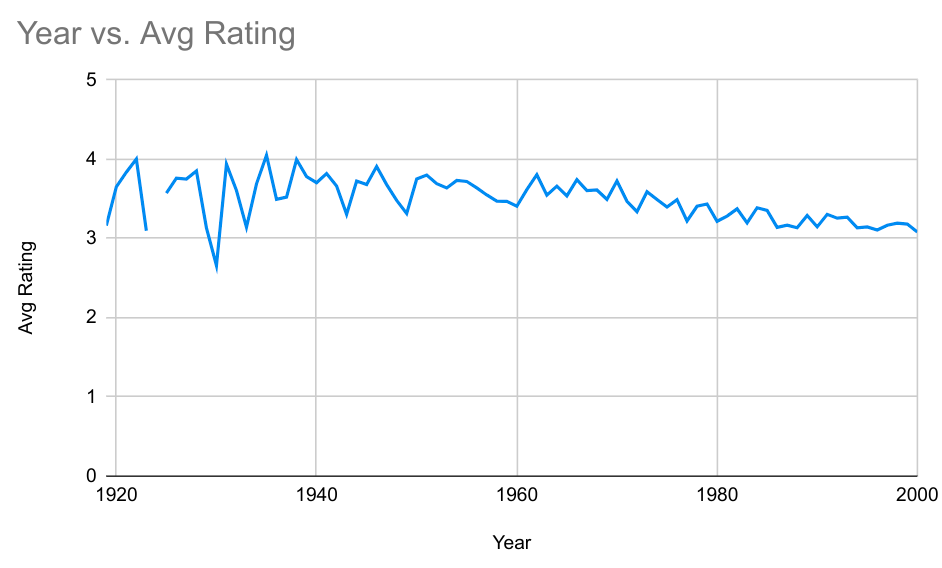
\includegraphics[width=0.5\textwidth]{year_vs_rating}
}{%    
    \caption[Year-of-release vs. Ratings]{Year-of-release vs. Ratings}
    \label{fig:year_vs_rating}
}

\capbtabbox{%
	\begin{tabular}{|l|l|l|l|}
	\hline
	\textbf{age} & \textbf{rating} & \multicolumn{1}{l|}{\textbf{gender}} & \multicolumn{1}{l|}{\textbf{rating}} \\ \hline
	18  & 3.621  & \multicolumn{1}{l|}{Female} & \multicolumn{1}{l|}{3.731}  \\ \hline
	25  & 3.668  & \multicolumn{1}{l|}{Male}   & \multicolumn{1}{l|}{3.692}  \\ \hline
	35  & 3.745  &                             &                             \\ \cline{1-2}
	45  & 3.771  &                             &                             \\ \cline{1-2}
	50  & 3.798  &                             &                             \\ \cline{1-2}
	56  & 3.833  & \multicolumn{1}{l|}{}       & \multicolumn{1}{l|}{}       \\ \hline
	\end{tabular}
}{%
	\caption[Age, Gender vs. Rating]{Age, Gender vs. Ratings}%
	\label{tab:table-6}
}
\end{floatrow}
\end{figure}

\textbf{1}. Old movies have higher average ratings (see \Cref{fig:year_vs_rating}). Female or elder users give higher average ratings (see \Cref{tab:table-6}).

Some possible interpretations to these phenomenons are that (1) people are more strict with new movies than old movies;
(2) people are usually nostalgia; (3) female users are more emotional than male users; (4) elder users are more generous on giving high ratings than young users.

\textbf{2}. Some users are too lazy to change default profiles.

Around 200 users (out of 3,706 users) have $age=1$ and $profession=0$.
These users are considered as abnormal data entries, which are ignored in the calculation of local deviations.

\subsection{Bigger Training Set}

Since there is only a limited amount of training data, an attempt of increasing training dataset was conducted.
More specifically, a new rating dataset was produced by adding the least RMSE submission to existing rating dataset.
As a result, the size of the rating dataset was increased 9.9\% to a total of 1,000,209 (`ratings.csv' 910,190 + `submission.csv' 90,019) entries.
However, a re-training and re-submission on the new rating dataset did not further minimize RMSE. The result was near 0.858, which was 0.004 higher than then optimal submission.

Although the result failed to meet expectation, the author still believes that an iterative training (i.e. update training set with the least RMSE submission) may enhance the result eventually.
Due to a lack of computational resources, the author cannot afford such experiment.

\newpage
\section{Conclusions and Future Works}

\subsection{Conclusions}

In this report, the objective was met.
An Item-Item Collaborative Filtering recommendation system was successfully developed, achieving a minimum RMSE of 0.84991 on the Kaggle public score board.
The important conclusions that can be drawn from the report are included below.

\textbf{1}. Larger $N$ improves RMSE, but there is a diminishing return.

\textbf{2}. It is critical to address cold-start problem.

\textbf{3}. Rounding is a bad idea.

\subsection{Future Works}

Some potential steps for future improvement of the work started by this report have been identified.

\textbf{1}. Develop local RMSE test.

Developing own local RMSE test will save a huge amount of time resource. The ratio of splitting limited training set into a new training set and own test set needs to be carefully chosen. 

\textbf{2}. Take movie names into consideration.

In the future, one may use techniques (such as TFIDF) to find correlation of movie names and ratings.
This may help enhancing the RMSE result.

\textbf{3}. Incorporate latent factor models.

Combining latent factors can further reduce RMSE, help achieving more accurate result.

%%%%%%%%%%%%%%%%%%%%%%%%%%%%%%%%%%%%%%%%%%%%%%%%%%%%%%%%%%%%%%%%%%%%%%%%%%%%%%%%
%% ************************************************************************** %%
%% *                               References                               * %%
%% ************************************************************************** %%
%%%%%%%%%%%%%%%%%%%%%%%%%%%%%%%%%%%%%%%%%%%%%%%%%%%%%%%%%%%%%%%%%%%%%%%%%%%%%%%%

\printbibliography[heading=none]

%%%%%%%%%%%%%%%%%%%%%%%%%%%%%%%%%%%%%%%%%%%%%%%%%%%%%%%%%%%%%%%%%%%%%%%%%%%%%%%%
%% ************************************************************************** %%
%% *                               Appendices                               * %%
%% ************************************************************************** %%
%%%%%%%%%%%%%%%%%%%%%%%%%%%%%%%%%%%%%%%%%%%%%%%%%%%%%%%%%%%%%%%%%%%%%%%%%%%%%%%%

%% appendices use section and subsection numbering
%\appendix
%
%\section{Title of First Appendix}
%\label{app:firstappx}
%Use the No Spacing style.
%
%\section{Another Appendix}
%\label{app:anotherappx}
%Again, use the no spacing style for appendices.

\end{document}
